\section{Methodology}\label{sec:methodology}

% 标题详细一点
\begin{figure*}[!t] % 移除了不支持的 h 和 b，优先放在顶部
    \centering
    \vspace{-10pt}
    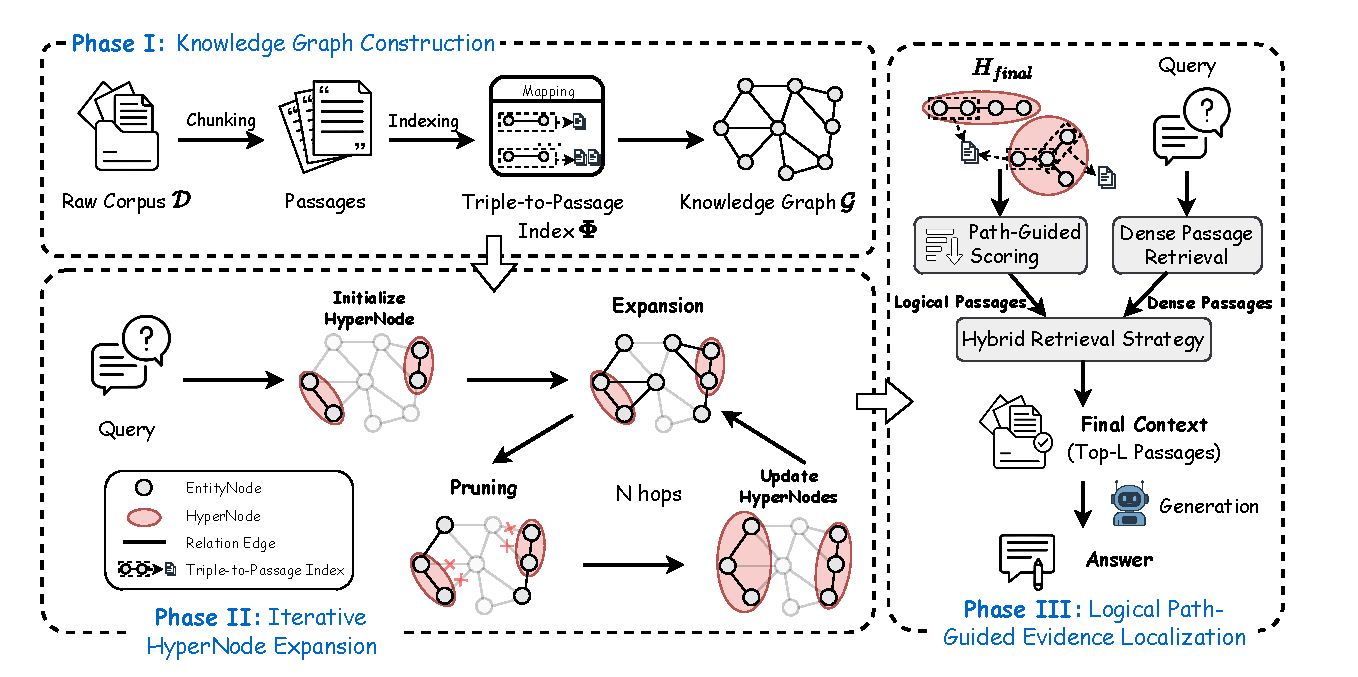
\includegraphics[width=0.95\textwidth]{figures/help_framework.pdf} % 建议简化文件名
    \vspace{-8pt}
    \caption{Overview of the HELP framework. The workflow consists of three stages: (I) Knowledge Graph Construction, utilizing OpenIE to build the Triple-to-Passage Index; (II) Iterative HyperNode Expansion, which iteratively chains triples as HyperNodes while pruning irrelevant ones to maintain reasoning coherence; and (III) Logical Path-Guided Evidence Localization, where HyperNodes are grounded back to the original passages for precise evidence retrieval via a hybrid mechanism.}
    \label{fig: HELP framework}
\vspace{-10pt}
\end{figure*}

%引一下 done
We elaborate on the mechanism of HELP, as illustrated in Fig.~\ref{fig: HELP framework}. Our approach comprises of three phases: Knowledge Graph Construction (Sec.~\ref{sec: knowledge_graph_construction}), Iterative HyperNode Expansion (Sec.~\ref{sec:hypernode_expansion}), and Logical Path-Guided Evidence Localization (Sec.~\ref{sec:evidence_localization}).
%. In Sec.~\ref{sec: knowledge_graph_construction}, we present the Knowledge Graph Construction, where we employ OpenIE to extract structured triplets from the raw corpus. In Sec.~\ref{sec:hypernode_expansion}, we elaborate on Iterative HyperNode Expansion, a process that constructs reasoning paths by dynamically expanding explicit nodes and relations. Finally, in Sec.~\ref{sec:evidence_localization}, we discuss the Logical Path-Guided Evidence Localization, which utilizes these HyperNodes as evidence to precisely retrieve passages from the raw corpus.


\subsection{Knowledge Graph Construction}\label{sec: knowledge_graph_construction}
% 可要可不要
To incorporate structural knowledge, Graph-Based RAG leverages a Knowledge Graph denoted as $\mathcal{G}=(\mathcal{V}, \mathcal{E})$, where $\mathcal{V}$ represents entities and $\mathcal{E}$ represents relations. The graph is typically constructed by extracting triplets from the corpus. Existing methods perform graph traversal, such as Personal PageRank or BFS, starting from entities mentioned in $q$. However, traversing the entire graph topology is computationally expensive, and ignoring edge semantics leads to accuracy loss. Our method aims to resolve this trade-off.

To bridge the gap between unstructured text and structured reasoning, we first construct a Knowledge Graph $\mathcal{G}$. Given a corpus of documents, we partition each document into passages $\mathcal{P} = \{p_1, p_2, \dots, p_N\}$. Then we employ an Open Information Extraction (OpenIE) module to extract a set of relational triplets from each passage $p_i$. Let $\mathcal{T}_i = \{ (h_k, r_k, t_k) \}_{k=1}^{|\mathcal{T}_i|}$ denote the sequence of relational triplets extracted from passage $p_i$.


Crucially, to support our retrieval mechanism, we construct a Triple-to-Passage Index $\Phi$, which captures graph-text correlations. For every unique triplet $\tau = (h, r, t)$, we maintain a mapping to its provenance passages:
\begin{equation}
    \Phi(\tau) = \left\{ (p_i, w_i) \mid \tau \in \mathcal{T}_i, \quad w_i = \frac{1}{|\mathcal{T}_i|} \right\}
\end{equation}
$w_i$ serves as a density-normalized weight, ensuring passages containing fewer yet more specific facts outweigh dense, noisy passages in retrieval scores.

\subsection{Iterative HyperNode Expansion}
\label{sec:hypernode_expansion}

To enable multi-hop reasoning, we introduce HyperNode Expansion, a strategy built upon the iterative merging and expanding of relational contexts. In our framework, a HyperNode $H = \{\tau_1, \dots, \tau_m\}$ is defined as a cumulative unit instantiated by merging $m$ coherent knowledge triplets into a unified semantic representation. By recursively expanding these nodes with adjacent relations, we transform discrete, isolated facts into integrated multi-hop reasoning paths.

\subsubsection{HyperNode Serialization}
% To map a HyperNode into a dense vector space, we must handle the permutation invariance of the set structure. We employ a deterministic linearization function $S(\cdot)$. We first sort the triplets lexicographically to ensure a unique order, and then flatten them into a single text sequence:
% \begin{equation}
%     S(H) = \text{join}\left( \bigcup_{\tau \in \text{sorted}(H)} \text{concat}(h_\tau, r_\tau, t_\tau) \right)
% \end{equation}
% The dense vector representation of the HyperNode is then obtained via an encoder: $v_{H} = E(S(H))$. This embedding captures the aggregate semantic context of the specific HyperNode.

To map a HyperNode into a dense vector space, we must handle the permutation invariance of the set structure. Unlike traditional sequential data, a HyperNode $H$ is an unordered set of triplets. Without a canonical ordering, the encoder $E(\cdot)$ might produce inconsistent embeddings for the same set of facts  in different sequences, hindering the effective representation of evidence within the structured data.

To mitigate this, we employ a deterministic linearization function $S(\cdot)$ designed to bridge the gap between structured sets and sequential modeling. Specifically, we first sort the triplets lexicographically based on their constituent elements to ensure a unique, reproducible order regardless of the original data extraction sequence. Once sorted, these structured components are flattened into a unified text sequence:
\begin{equation}
    S(H) = \text{join}\left( \bigcup_{\tau \in \text{sorted}(H)} \text{concat}(h_\tau, r_\tau, t_\tau) \right)
\end{equation}
The dense vector representation of the HyperNode is then obtained via a pre-trained Transformer-based encoder: $v_{H} = E(S(H))$. By mapping the relational structure into a continuous latent space, this process allows the model to capture the aggregate semantic context. 

\subsubsection{Iterative Expansion Process}
The core of our approach is the iterative expansion mechanism. Given a user query $q$, we first map it to a normalized vector representation $v_q = \frac{E(q)}{\|E(q)\|_2}$, where $E(\cdot)$ denotes the encoder. The expansion process then updates the set of active HyperNodes over $N$ hops to generate the final set $H_{final}$. The overall procedure is summarized in Algorithm \ref{alg:hypernode_expansion} and details are provided below.


\textbf{HyperNode Initialization.} It begins with the identification of seed HyperNodes, which serve as the semantic anchors for subsequent reasoning. Instead of starting from raw entities, we leverage the fine-grained semantics of individual triplets $\{\tau\}$ extracted from the corpus. We compute the cosine similarity between the query vector $v_q$ and the normalized embedding of each candidate triplet. By selecting the top-$n$ triplets with the highest alignment scores, we form the initial set $H_{1}$. This step ensures that the expansion starts from the most promising factual kernels, effectively reducing the noise introduced by irrelevant graph regions.

% \textbf{Iterative Expansion.} At each step $i$ (where $2 \le i \le N$, and $N$ denotes the number of expansion hops), the model extends the reasoning paths inherited from the previous step to incorporate broader context. Specifically, in the $i$-th expansion round, for each HyperNode $H \in H_{i-1}$, we perform a neighborhood traversal within the Knowledge Graph $\mathcal{G}$. By examining the local topology of the graph, we identify a set of adjacent triplets $\mathcal{T}_{adj}$ that share at least one entity with the current components of $H$. We then generate a set of expanded candidate HyperNodes $\mathcal{C}_{cand}$ by performing a union operation: $H' = H \cup \{\tau_{next}\}$, where $\tau_{next} \in \mathcal{T}_{adj}$. This incremental growth allows the HyperNode to transition from a single fact to a complex path structure representing a multi-hop chain of evidence.

\textbf{Iterative Expansion.} At each step $i$ (where $2 \le i \le N$, and $N$ denotes the number of expansion hops), the model extends reasoning paths to incorporate broader context. Specifically, in the $i$-th expansion round, we process each HyperNode $H \in H_{i-1}$ individually. We identify a set of adjacent triplets $\mathcal{T}_{adj}$ from the Knowledge Graph $\mathcal{G}$ that are directly connected to the entities contained within the current $H$. For each adjacent triplet $\tau_{next} \in \mathcal{T}_{adj}$, we instantiate a new expanded HyperNode $H' = H \cup \{\tau_{next}\}$. The global candidate set $\mathcal{C}_{cand}$ is then formed by accumulating all such generated $H'$ instances derived from each preceding HyperNode in $H_{i-1}$. This incremental growth allows each HyperNode to transition from a single fact to a complex path structure representing a multi-hop chain of evidence.

% \textbf{Iterative Expansion.} At step $i$ (where $2 \le i \le N$), the model extends reasoning paths to incorporate broader context. Specifically, we process each HyperNode $H \in H_{i-1}$ individually. We identify adjacent triplets $\mathcal{T}_{adj}$ from $\mathcal{G}$ directly connected to entities in $H$. For each $\tau_{next} \in \mathcal{T}_{adj}$, we instantiate a new HyperNode $H' = H \cup \{\tau_{next}\}$. The global candidate set $\mathcal{C}_{cand}$ is formed by accumulating all $H'$ instances derived from each base HyperNode. This incremental growth transitions single facts into complex multi-hop evidence chains.

\textbf{Pruning via Semantic Distance.} To counteract the exponential growth of the search space and to maintain focus on the query's core intent, we implement a semantic-guided beam search strategy. This strategy ensures that only the most semantically pertinent reasoning paths are retained at each hop. We serialize the content of each candidate $H'$ into a sequence $S(H')$ and compute its distance to the query. Since the embeddings are normalized, we utilize the Euclidean distance as our metric:
\begin{equation}
    \label{eq:dist_metric}
    \text{dist}(H', q) = \left\| \frac{E(S(H'))}{\|E(S(H'))\|_2} - v_q \right\|_2
\end{equation}
Based on Eq. \eqref{eq:dist_metric}, we select the top-$k$ HyperNodes with the minimal distance to form $H_{i}$. By maintaining a fixed beam width $k$, it constrains the search space to a manageable scale, preventing the computational overhead typically associated with deep graph traversals. Consequently, it ensures that the final converged set, $H_{final}$, is not merely a collection of isolated facts, but a structured assembly of complete, logically coherent, and semantically aligned reasoning paths tailored to the specific information need.

\begin{algorithm}[!tb]
\caption{Iterative HyperNode Expansion Algorithm}
\label{alg:hypernode_expansion}
\begin{algorithmic}[1]
\REQUIRE User query $q$, Knowledge Graph $\mathcal{G}$, Expansion hops $N$, Initial triple size $n$, Beam size $k$
\ENSURE Final set of HyperNodes $H_{final}$

\STATE \textbf{Initialize:} $v_q \leftarrow \text{Normalize}(E(q))$

\STATE \textit{// Step 1: Initialization with Seed HyperNodes}
\STATE Retrieve all triples $\{\tau\}$ from $\mathcal{G}$
\STATE Score triples by similarity to $v_q$
\STATE $H_1 \leftarrow \text{Top-}n \text{ ranked triples}$

\STATE \textit{// Step 2: Iterative Expansion Process}
\FOR{$i = 2$ to $N$}
    \STATE $\mathcal{C}_{cand} \leftarrow \emptyset$ 
    
    \FOR{each HyperNode $H$ in $H_{i-1}$}
        \STATE $\mathcal{T}_{adj} \leftarrow \{ \tau \in \mathcal{G} \mid \tau \text{ is adjacent to entities in } H \}$
        \FOR{each $\tau_{next}$ in $\mathcal{T}_{adj}$}
            \STATE \textbf{Expand:} $H' \leftarrow H \cup \{ \tau_{next} \}$
            \STATE Add $H'$ to $\mathcal{C}_{cand}$
        \ENDFOR
    \ENDFOR
    
    \STATE \textit{// Step 3: Pruning (Beam Search)}
    \STATE $H_{i} \leftarrow \emptyset$
    \FOR{each candidate $H'$ in $\mathcal{C}_{cand}$}
        \STATE  $v_{H'} \leftarrow \text{Normalize}(E(S(H')))$
        \STATE \textbf{Score:} Calculate $\text{dist}(H', q)$ using Eq. \eqref{eq:dist_metric}
    \ENDFOR
    
    \STATE $H_{i} \leftarrow$ Select top-$k$ HyperNodes from $\mathcal{C}_{cand}$ with minimal distance
\ENDFOR

%\STATE $H_{final} \leftarrow H_{N}$
\STATE \textbf{return} $H_{final} = H_{N}$
\end{algorithmic}
\vspace{-2pt}
\end{algorithm}


\subsection{Logical Path-Guided Evidence Localization}
\label{sec:evidence_localization}

The final phase of our framework is Logical Path-Guided Evidence Localization, a process designed to transform abstract structural information into concrete textual evidence. By utilizing the expanded HyperNodes as precise semantic anchors, we can pinpoint the most relevant supporting passages within the massive corpus, ensuring that the downstream generation is grounded in verified facts.

To bridge the semantic gap between the retrieved structural knowledge and the original source corpus, we leverage the Triple-to-Passage Index $\Phi$. This specialized inverted index, as constructed in Sec.~\ref{sec: knowledge_graph_construction}, establishes a one-to-many mapping between each unique triplet $\tau$ and the set of source passages from which it was extracted. By recognizing that a single factual claim can be instantiated across multiple disparate passages, this index ensures comprehensive evidence coverage. Such a mechanism enables robust provenance tracking, allowing the model to backtrack from a specific hop in the reasoning path to all supporting textual fragments that validate the underlying logic.

We compute a relevance score for each passage $p$ by aggregating the evidentiary signals from the complete set of reasoning paths. Instead of considering only unique triplets, we sum the contributions of all triplets $\tau$ across the final set of HyperNodes $H_{final}$ to account for the consensus of evidence. The relevance score for passage $p$ is derived as:
\vspace{-2pt}
% \begin{equation}
%     \small
%     \text{Score}(p) = \sum_{H \in H_{final}}\sum_{\tau \in H} \mathbb{I}(p \in \Phi(\tau)) \cdot e^{-\text{dist}(\tau, q)} \cdot w_{p,\tau}
% \end{equation}
\begin{equation}
    \small
    \text{Score}(p) = \sum_{H \in H_{final}} \sum_{\tau \in H} \mathbb{I}(p \in \Phi(\tau)) \cdot e^{-\text{dist}(H, q)} \cdot w_{p, \tau}
\end{equation}
where $w_{p,\tau}$ represents the provenance weight associated with the extraction density, as mentioned in Sec.~\ref{sec: knowledge_graph_construction}.

In this formulation, the term $\kappa(H, q) = e^{-\text{dist}(H, q)}$ functions as a non-linear soft-matching mechanism. 
By aggregating scores across all HyperNodes, this approach naturally yields a consensus-based ranking: passages are scored higher not only for semantic alignment with the query, but also for being repeatedly reinforced through multiple distinct reasoning paths.
%By aggregating scores across all HyperNodes, this approach naturally implements a consensus-based ranking: a passage receives a higher score not only if it is semantically aligned with the query, but also if it is repeatedly reinforced by multiple distinct reasoning paths. 
This ensures that the evidence localization is robust to individual triplet noise and favors passages that reside at the intersection of diverse logical chains.

Drawing inspiration from hybrid search paradigms \cite{bhagdev2008hybrid, wang2025balancing}, we adopt a composite strategy to construct a robust final context of size $K$. We recognize that Logical Path-Guided Evidence Localization and Dense Passage Retrieval (DPR) operate on distinct and complementary relevance signals. Our logical path-guided approach ensures high precision by leveraging the consensus of multi-hop reasoning chains: passages that are reinforced by multiple intersecting paths receive prioritized ranking through our additive scoring mechanism. In contrast, DPR excels at capturing broad semantic coverage that structural methods might overlook.

To leverage this complementarity, we assign a primary quota of $M$ passages to the evidence localized via the Logical Path-Guided Evidence Localization, ensuring the final context is anchored in structured reasoning. This foundation is then supplemented with top-ranked candidates from DPR to fill the remaining slots, with a deduplication step to maximize incremental information gain. As demonstrated in our ablation study (see Sec.~\ref{sec: hybrid strategy}), this hybrid retrieval strategy—prioritizing structure-based consensus while backfilling with semantic matches—yields superior performance compared to single-stream methods by balancing the depth of logical rigor with the breadth of semantic recall.